% !TEX root = ../tfg.tex

Este capítulo presenta los datos sobre los que se apoya el trabajo.
Se parte de dos conjuntos de datos públicos.
El primero reúne vídeos de partidos con el instante de cada golpe y el segundo aporta la posición de la pelota.
A ellos se suma un etiquetado propio, que fue necesario para identificar qué tipo de golpe es.
Además, esta información resulta imprescindible para entrenar el clasificador, y por eso hubo que crearla a mano.
El capítulo termina con un resumen de los datos que utiliza cada modelo del sistema.

\section{Conjunto de datos CVSPORTS}
\label{sec:cvsports}

El punto de partida del trabajo es el conjunto de datos que publicaron Decorte \textit{et al.}~\cite{decorte2024padel} con el nombre de Padel Hit Detection Dataset.
En esta memoria se denomina CVSPORTS, por el taller en el que se presentó, y es la base de la mayor parte del sistema.
Contiene 99 puntos tomados de los resúmenes de las retransmisiones de 11 torneos, grabados con la cámara de la propia emisión y con su audio.

Las anotaciones del conjunto son de dos clases.
De cada uno de los 2377 golpes se conoce el momento en que empieza y termina su sonido, lo que permite entrenar y evaluar la detección de los golpes.
Además, en 16 puntos de Vigo se indica el jugador que ejecuta cada golpe.
Son los únicos del conjunto que lo incluyen, por lo que son también los únicos con los que se puede medir si el sistema atribuye bien cada golpe.

La \cref{tab:dataset} muestra cómo se reparten los puntos y los golpes entre los torneos, junto con su entorno.

\begin{table}[htbp]
  \centering
  \caption{Puntos, golpes y entorno de cada torneo de CVSPORTS.}
  \label{tab:dataset}
  \begin{tabular}{lrrl}
\toprule
\textbf{Torneo} & \textbf{Puntos} & \textbf{Golpes} & \textbf{Entorno} \\
\midrule
Finlandia & 10 & 320 & Interior \\
Vigo & 17 & 315 & Exterior \\
Madrid & 11 & 296 & Interior \\
Bruselas & 12 & 250 & Exterior \\
Alemania & 7 & 227 & Interior \\
Málaga & 10 & 201 & Interior \\
Ámsterdam & 9 & 190 & Interior \\
Menorca & 6 & 187 & Interior \\
Malmö & 7 & 173 & Interior \\
Valladolid & 6 & 114 & Exterior \\
Valencia & 4 & 104 & Interior \\
\midrule
\textbf{Total} & \textbf{99} & \textbf{2377} &  \\
\bottomrule
\end{tabular}

\end{table}

\section{Conjunto de datos PadelTracker100}
\label{sec:padeltracker}

CVSPORTS permite entrenar la detección de los golpes pero no incluye ninguna anotación de la pelota.
Esta información es necesaria para atribuir cada golpe a un jugador y para clasificarlo, y por eso se recurrió a un segundo conjunto de datos llamado PadelTracker100~\cite{badanerin2026padeltracker100}.
Este conjunto lo forman dos finales del World Padel Tour disputadas en Barcelona en 2022 y fue publicado por NTT Data y la Universidad de Oviedo.

De este conjunto se ha utilizado la posición de la pelota, que está anotada mediante una caja en los fotogramas en los que es visible.
Las dos finales cumplen funciones distintas, ya que la masculina, con \num{19320} fotogramas con la pelota anotada, sirve para entrenar el detector y la femenina, con \num{37904}, para evaluarlo.
De este modo la medida se obtiene sobre un partido que el modelo no ha visto durante el entrenamiento.

Esta forma de evaluar tiene sin embargo un límite.
Ambas finales se jugaron en la misma pista y con la misma cámara, de modo que los resultados no permiten saber cómo se comportaría el detector en otras condiciones (\cref{cap:resultados}).

\section{Etiquetado del tipo de golpe}
\label{sec:etiquetado}

El clasificador aprende a partir de ejemplos que tengan etiquetado el tipo de golpe. Fue necesario por tanto etiquetar uno a uno los 2377 golpes del conjunto de datos de CVSPORTS.

Para etiquetar los golpes no hizo falta recorrer los vídeos enteros, porque ya incluyen el instante de cada uno.
El etiquetado consiste por tanto en ir directamente a cada instante anotado y elegir el tipo del golpe.
Esto acelera el etiquetado, ya que localizar cada golpe dentro de un vídeo completo es una tarea tediosa.

Para etiquetar se desarrolló una herramienta propia.
La primera versión mostraba solo el fotograma del instante de cada golpe, pero al usarla resultaba difícil saber de qué tipo era.
La razón es que un golpe no se define por la posición del cuerpo en un instante sino por el movimiento completo, desde que el jugador se prepara hasta que termina el gesto.
Por ello, la herramienta pasó a reproducir en bucle y a velocidad real una ventana de vídeo antes y después del golpe, y con ello facilita su clasificación.
La \cref{fig:herramienta} muestra la interfaz, en la que cada golpe se etiqueta pulsando una sola tecla.

\begin{figure}[H]
  \centering
  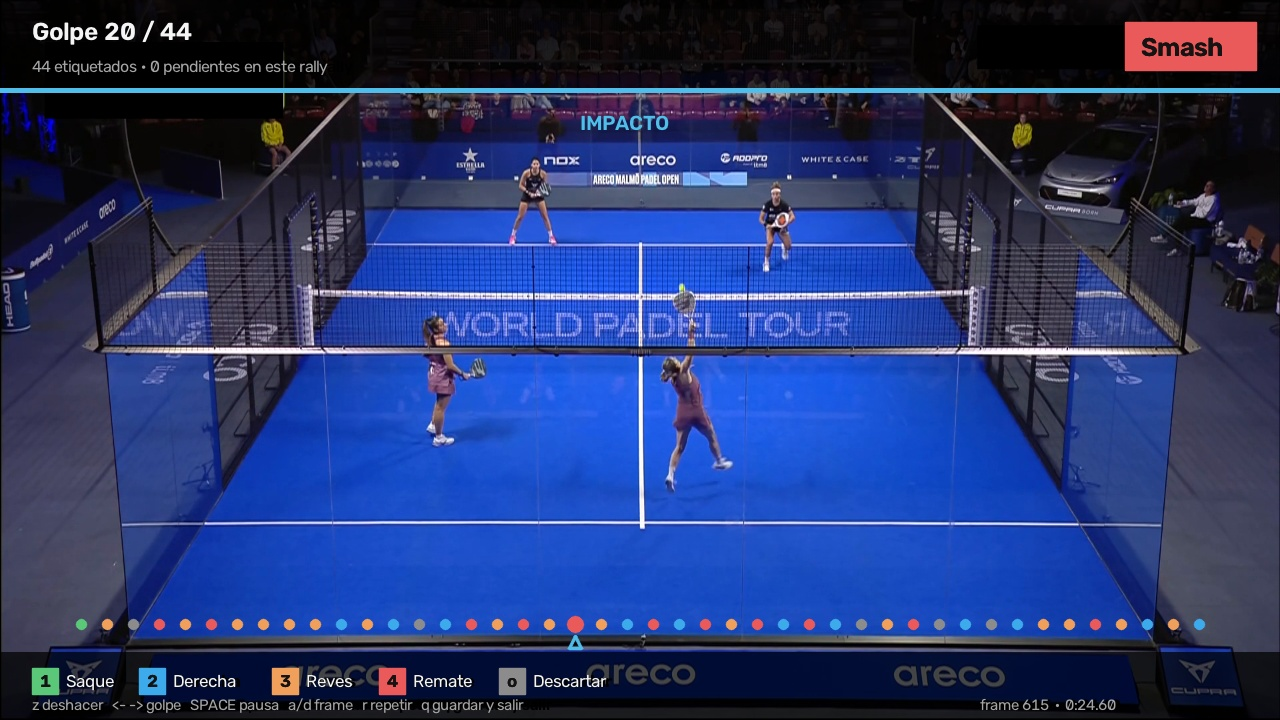
\includegraphics[width=0.85\textwidth]{figuras/capturas/herramienta-etiquetado}
  \caption{Herramienta de etiquetado en el instante de un remate: arriba, el golpe dentro del punto y su etiqueta; abajo, un círculo por cada golpe del punto, con el color de su clase, y la tecla de cada clase.}
  \label{fig:herramienta}
\end{figure}

Cada golpe se etiqueta con una de estas cuatro clases:
\begin{itemize}
  \item La derecha es un golpe que el jugador ejecuta con la pelota en el lado de la mano con la que sostiene la pala. Es el golpe más natural y el que más se repite durante un punto.
  \item El revés es un golpe que se ejecuta con la pelota en el lado opuesto a la mano que sostiene la pala. Obliga al jugador a girar el cuerpo y a cruzar el brazo por delante para alcanzarla.
  \item El remate es un golpe que se ejecuta por encima de la cabeza, con el brazo extendido e impactando en el punto más alto. Suele utilizarse para responder a los globos del rival y busca potencia o colocación.
  \item El saque es el golpe con el que empieza cada punto. El jugador deja botar la pelota, la golpea por debajo de la cintura y debe enviarla en diagonal a la zona de saque del rival, por lo que solo hay uno por punto.
\end{itemize}
Cuando un golpe no encaja en ninguna de las cuatro clases se anota como ``otro''.
Es el caso de los gestos atípicos y también de los golpes que no pueden etiquetarse con seguridad.

Estas cuatro clases se eligieron por ser las familias básicas de golpes del pádel y se definen por el gesto con el que se ejecuta el golpe.
La \cref{tab:etiquetado} muestra el resultado del etiquetado.
La derecha y el revés son las clases más frecuentes y representan cerca de un tercio de los golpes cada una, mientras que el remate supone casi la cuarta parte.
El saque es la clase con menos ejemplos.
Aparte de estas cuatro clases, los golpes anotados como ``otro'' representan un 7~\% del total.
Es una proporción pequeña, de modo que al descartarlos del entrenamiento se conserva la gran mayoría de los datos.

\begin{table}[htbp]
  \centering
  \caption{Reparto del etiquetado propio por tipo de golpe.}
  \label{tab:etiquetado}
  \begin{tabular}{lcc}
\toprule
\textbf{Clase} & \textbf{Golpes} & \textbf{Porcentaje} \\
\midrule
Derecha & \num{813} & \SI{34.2}{\percent} \\
Revés & \num{735} & \SI{30.9}{\percent} \\
Remate & \num{565} & \SI{23.8}{\percent} \\
Saque & \num{97} & \SI{4.1}{\percent} \\
Otro & \num{167} & \SI{7.0}{\percent} \\
\midrule
Total & \num{2377} &  \\
\bottomrule
\end{tabular}

\end{table}

\section{Uso de los datos en cada modelo}
\label{sec:uso-datos}

Una vez presentados los datos, conviene ver cómo se reparten entre los componentes del sistema, porque no todos los utilizan de la misma manera.
La \cref{tab:uso-datos} resume qué datos intervienen en cada componente y con qué fin.

\begin{table}[htbp]
  \centering
  \caption{Datos que utiliza cada componente del sistema.}
  \label{tab:uso-datos}
  \small
  \begin{tabular}{p{3.8cm}p{5.4cm}p{4.8cm}}
\toprule
\textbf{Componente} & \textbf{Datos} & \textbf{Uso} \\
\midrule
Detector de golpes & CVSPORTS (audio e instantes) & Entrenamiento y evaluación \\
Detector de la pelota & PadelTracker100 (dos finales) & Entrenamiento y evaluación \\
Asignación del golpe & CVSPORTS (Vigo) & Evaluación \\
Clasificador del tipo & Etiquetado propio & Entrenamiento y evaluación \\
\bottomrule
\end{tabular}

\end{table}
